%\documentclass[handout, 8pt]{beamer}
\documentclass[8pt]{beamer}

\usetheme{Singapore}
\usefonttheme{serif} 


%%%%%%%%%%%%%%%%%%%%%%%%
% Usual LaTeX Packages %
%%%%%%%%%%%%%%%%%%%%%%%%
\usepackage{pdfpages}
\usepackage{amsmath}
\usepackage{amscd}
\usepackage{amsfonts}
\usepackage{amssymb}
\usepackage{graphicx}
\usepackage{mathrsfs} 			% For Weinberg-esque letters
\usepackage{cancel}				% For "SUSY-breaking" symbol
\usepackage{slashed}            % for slashed characters in math mode
\usepackage{bbm}                % for \mathbbm{1} (unit matrix)
\usepackage{dsfont}
\usepackage{amsthm}				% For theorem environment
\usepackage{multirow}			% For multi row cells in table
\usepackage{arydshln} 			% For dashed lines in arrays and tables
\usepackage{multirow}
\usepackage{multicol}
\usepackage{bigstrut}
\usepackage{setspace}
\usepackage{endnotes}
\usepackage{etex}
\usepackage{lmodern}
\usepackage{booktabs}
\usepackage{graphics}
\usepackage[flushleft]{threeparttable}
%\usepackage{enumitem}
%\setlist[itemize]{itemsep=2mm}
\usepackage{array}
\usepackage{color}
\usepackage{colortbl}
\usepackage{hyperref}
\usepackage{ifplatform}
\usepackage{dcolumn}
\usepackage{threeparttable}
\usepackage{hyperref}
\usepackage{tabularx}
\usepackage{soul}
\usepackage{ulem}

\usepackage[utf8]{inputenc}
\usepackage[T1]{fontenc}
\usepackage{appendixnumberbeamer}
\usepackage{xcolor}
\def\boxit#1{%
  \smash{\color{red}\fboxrule=1pt\relax\fboxsep=2pt\relax%
  \llap{\rlap{\fbox{\vphantom{0}\makebox[#1]{}}}~}}\ignorespaces
}
\usepackage{appendixnumberbeamer}

\newcommand{\E}{\mathbb{E}}

% Code for Hiding Columns in Tables
\newcolumntype{H}{>{\setbox0=\hbox\bgroup}c<{\egroup}@{}}


\graphicspath{{images/}}	% Put all images in this directory. Avoids clutter.





% BIBLIOGRAPHY (OPTION: BIBLATEX) ===========================================
\usepackage{csquotes}
\usepackage[natbib = true, backend = biber, style  = authoryear-icomp]{biblatex}
\addbibresource{References.bib}

\usepackage{setspace}
\setbeamercovered{transparent}

%gets rid of navigation symbols
\setbeamertemplate{navigation symbols}{}

\setbeameroption{show notes}
%\setbeameroption{show only notes}
%\setbeameroption{hide notes}

% A simple slide counter at the bottom of the slide
\setbeamertemplate{footline}{
   \begin{beamercolorbox}[ht=4ex,leftskip=0.3cm,rightskip=0.3cm]{author in head/foot}
    \vspace{0.1cm}
    \hfill \insertframenumber / \inserttotalframenumber
  \end{beamercolorbox}
   \vspace*{0.1cm}
} 

\newcommand\independent{\protect\mathpalette{\protect\independenT}{\perp}}
\def\independenT#1#2{\mathrel{\rlap{$#1#2$}\mkern2mu{#1#2}}}

\setbeamercovered{transparent}


\title{The limits of self-commitment and private paternalism \\
Preliminary --comments welcome}
\author{Craig McIntosh \and Isaac Meza \and Joyce Sadka \and Enrique Seira \and Francis J.\ DiTraglia }

\date{February 2023}

%\setbeamercolor{section in head/foot}{bg=darkcrimsonred}
\setbeamersize{text margin left=11pt, text margin right=11pt}
%\setbeamertemplate{section in toc}[square]




%%%%%%%%%%%%%%%%%%%%%%%%%%%%%%%%%%%%%%%
%%%%%%%%%%%%%%%%%%%%%%%%%%%%%%%%%%%%%%

\begin{document}


\begin{frame}[c, noframenumbering]%{\phantom{title page}}
% The \phantom{title page} is a kludge to get the red bar on top
\titlepage
\end{frame}


\section{Motivation}



\begin{frame}{Motivation: Private paternalism}
\begin{itemize}
    \vfill \item Many institutions —firms, schools, financial contracts— restrict choice using built-in commitment mechanisms which help workers, students, borrowers overcome self-control problems
    \begin{itemize}
        \item Loans with fixed repayment schemes, homework due dates, etc.
    \end{itemize}
    \vfill \pause\item At the same time these firms hide these forcing mechanisms and don’t market their commitment features, potentially because demand for them is low.
    \vfill  \item  Laibson (2018) argues that clients that benefit from commitment may underestimate its value, and that in such cases private paternalism could be beneficial.
    \vfill  \pause\item  We study the benefits of imposing a structured repayment contract, whether there is demand for it, and whether non-takers of such a commitment product would benefit from taking it.
\end{itemize}

\end{frame}

\section{Context}
\begin{frame}{Context - \textbf{Pawn}shops}
\begin{itemize}
    \vfill \item Pawn loans involve borrowers leaving valuable liquid assets as collateral in exchange for an immediate cash loan
    \vfill \pause \item The loan is overcollateralized (loan is 70\% of appraised value) and collateral is liquid.
    \begin{itemize}
        \item The lender approve loans in a few minutes without income or credit history check $\rightarrow$ used for emergencies.
    \end{itemize}

    \vfill \pause \item Controversial: interest rates and default rates are high, and used by people in distress.
    \vfill \pause \item Regulators believe mostly unsophisticated borrowers use it.
\end{itemize}
\end{frame}




\begin{frame}{Context}
\begin{columns}
\begin{column}{.45\textwidth}

\begin{figure}[H]
    \begin{center}
    \caption{Pawnshop}
        \includegraphics[width=0.95\textwidth]{Figuras/empenio2.png}
    \end{center}
    \end{figure}
\begin{figure}[H]
    \begin{center}
    \caption{Appraiser/tellers inside a pawnshop}
        \includegraphics[width=0.95\textwidth]{Figuras/empenio9.png}
    \end{center}
    \end{figure}    
    
    \end{column}
    
\begin{column}{.45\textwidth}

\begin{figure}[H]
    \begin{center}
    \caption{Pawnshop}
        \includegraphics[width=0.95\textwidth]{Figuras/empenio11.png}
    \end{center}
    \end{figure}
\begin{figure}[H]
    \begin{center}
    \caption{Lost pawns which are for sale}
        \includegraphics[width=0.95\textwidth]{Figuras/empenio3.png}
    \end{center}
    \end{figure}    
    
    \end{column}    
    \end{columns}
\end{frame}






\begin{frame}{Pawn contract}
    \begin{figure}[H]
    \label{ExplanatoryMaterial}
    \begin{center}
        \includegraphics[width=0.45\textwidth]{Figuras/sq_contract.png}
    \end{center}
\end{figure}
\end{frame}




\begin{frame}{Structured payments contract}
   \begin{itemize}
       \vfill \item We designed a new contract that is identical to the status quo contract except that it enhances the regularity and salience of payments as a way to encourage repayment.
         \begin{figure}[H]
    \label{ExplanatoryMaterial}
    \begin{center}
        \includegraphics[width=0.40\textwidth]{Figuras/fc_contract.png}
    \end{center}
\end{figure}
       
   \end{itemize}
    
\end{frame}

\section{Contribution}

\begin{frame}{Methodological Contribution}
\begin{itemize}
 \vfill \item A context of particular interest to behavioral literature:  the demand for commitment in financial contracts (Laibson 1997, Bryan et al. 2010).
 
   \vfill \pause  \item How do treatment effects relate to selection?  Key question in many literatures:
	\begin{itemize} 
		\item HTEs, MTE, LATEs, what is learned from IV regressions (Heckman \& Vytlacil, 2005).
		\item Health effects of universal versus elective interventions
		\item Optimal targeting (Alatas et al. 2012)
	\end{itemize}
    
    
  \vfill \pause  \item Three-arm design:  Control, Choice (voluntary takeup=ITT), Forcing (universal=ATE).  We illustrate how to use standard exclusion restrictions for point identification:
    \begin{itemize}
        \item Treatment on the Treated (ToT) and 
        \item Treatment on the Untreated (TUT), also
	\item Average Selection on Gains, Average Selection Bias, and Average Selection on Levels
    \end{itemize} 
    
  
     \vfill \pause  \item Key quantity in debate about paternalism:  impacts on those who wouldn't elect to take the program versus impacts on those that do.
    
   \vfill   \pause  \item Consider winners and losers from paternalism 
\end{itemize}
\end{frame}




\section{Design}

% \begin{frame}{Data}
% \begin{itemize}
%     \item Administrative data: XX months before and XX months after the experiment ended
%     \begin{itemize}
%         \item Unique identifier for each client and for the piece.
%         \item Value of the item, money loaned (70\%), date of pawning
%         \item For all payments: date and amounts
%         \item Fees incurred
%         \item Whether the client lost the pawn, renewed the contract
%     \end{itemize} 

%     \vfill \item Survey data
%     \begin{itemize}
%         \item During experiment, we asked clients to complete a 5-minute survey before going to the teller window to appraise their piece and before treatment status was known to them.
%         \item Demographics, proxies for income/wealth, education, present-biased preferences, experience pawning, if family or friends commonly asked for money, cost of going to branch, the subjective probability of recovering, the subjective value, etc.
%     \end{itemize}
% \end{itemize}    
% \end{frame}


\begin{frame}{Main outcomes: financial cost and default}
\label{fc_cost}
\begin{itemize}
    \item We are interested in measuring the   \hyperlink{fc_dist}{\beamerbutton{financial cost}}  of borrowing, which very saliently includes the cost of defaulting on the loan and losing the pawn.
    % \item We will measure loan default using an indicator $\mathds{1}(\text{Default}_i)$, and the cost in pesos using the following definition that capture borrower outlays:
\end{itemize}

   \begin{equation*}
    \text{Financial Cost}_i =  \underbrace{\sum_t P^i_{it}}_{\text{Pay to Interest}} + \underbrace{\sum_t P^f_{it}}_{\text{Pay to Fees}}  + \mathds{1}(\text{Default}_i) \times \left[\text{Pawn Val}_i + \underbrace{\sum_t P^c_{it}}_{\text{Pay to Capital}} \right]
   \end{equation*}

% \begin{itemize}
%     \vfill \item Towards the end of the presentation we will show results that apply a time discount factor.

% \end{itemize}
\end{frame}


% \begin{frame}{Distribution of APR}
% \vspace{.2in}
% \begin{equation*}
%     (\text{APR})_i =\left( 1 + \frac{\frac{\text{Financial Cost}_i}{\text{Appraised Value}_i}}{\text{loan term}_i}\right)^{\text{loan term}_i}-1
% \end{equation*}
% \vspace{.2in}
% \begin{figure}
%      \centering
%         \includegraphics[width=.75\textwidth]{Figuras/hist_apr.pdf}
%     \end{figure}
% \end{frame}

    
%\begin{frame}{Measuring Borrowers Financial Cost}
%\begin{columns}
%\begin{column}{.5\textwidth}
%    \begin{figure}[H]
%     \caption{Financial cost (MXN)}
%    \begin{center}
%    \includegraphics[width=\textwidth]{Figuras/hist_fc.pdf}
%    \end{center}
%    \end{figure}
%    \resizebox{1.0\linewidth}{!}{
%  \begin{minipage}{\linewidth}
%    \tiny{
    %\begin{align*}
    %\text{Financial Cost}_i =&  \underbrace{\sum_t P^i_{it}}_{\text{Pymnts to interests}} + \underbrace{\sum_t P^f_{it}}_{\text{Pymnts of fees}} \\
  %& + \underbrace{\mathds{1}(\text{Default}_i) \times (\text{Appraised Value}_i}_{\text{Cost of losing pawn}} + \underbrace{\sum_t P^c_{it}}_{\text{Pymnts to capital}})
%\end{align*}
%}
%  \end{minipage}
%}

%\end{column}
%\begin{column}{.5\textwidth}
%    \begin{figure}[H]
%     \caption{Effective APR}
%    \begin{center}
%    \includegraphics[width=\textwidth]{Figuras/hist_apr.pdf}
%    \end{center}
%    \end{figure}
%    \resizebox{.95\linewidth}{!}{
%  \begin{minipage}{\linewidth}    
%    \tiny{
    %\begin{align*}
    %(\text{APR})_i =&\left( 1 + \frac{\frac{\text{Financial Cost}_i}{\text{Appraised Value}_i}}{\text{loan term}_i}\right)^{\text{loan term}_i}-1 \\
   % & \\
   % & \\
   % & \\
   % &
%\end{align*}
%}
 % \end{minipage}
%}
%\end{column}
%\end{columns}
%\end{frame}




\begin{frame}{Treatment arms}
   \begin{itemize}
    \vfill \item Randomization at the branch-day level. 
    \begin{itemize}
        \vfill \item Control arm 
       \vfill \item Forced Commitment arm
       \vfill \item Choice Commitment arm
    \end{itemize}
    \vfill \pause \item The  existence  of  a  choice  arm  allows  us  not  only  to  measure  if  there  is  demand  for  such  a contract, but who demands it, not only in demographic terms, but in terms of potential treatment effects.
   \vfill \pause \item  This design is innovative and critical for our purposes, as it enables us to explore whether or not forcing people into a structured payment contract could be more beneficial than allowing choice for a significant fraction of them.
\end{itemize}
\end{frame}


% \begin{frame}{Description}

% \begin{figure}[H]
%      \caption{Experiment description}
%     \label{exp_description}
% \begin{center}
%         \includegraphics[width=0.85\textwidth]{Figuras/consort.pdf}
%   \end{center}
% \end{figure}

% \end{frame}







\section{Main Results}
\begin{frame}{Main results}

\begin{table}[H]
\caption{Main treatment effects}
\label{main_impact_table}
\begin{center}
\resizebox{0.95\textwidth}{!}{
\scriptsize{% Table generated by Excel2LaTeX from sheet 'decomposition_main_te_pres1'
\begin{tabular}{lcccccccc}
\toprule
      &       & \multicolumn{5}{c}{Components of FC}  &       &  \\
\cmidrule{3-7}      & FC    & \textcolor[rgb]{ .749,  .749,  .749}{Int. pymnt} & \textcolor[rgb]{ .749,  .749,  .749}{Fee pymnt} & \textcolor[rgb]{ .749,  .749,  .749}{Princ. pymnt} & \textcolor[rgb]{ .749,  .749,  .749}{Lost pawn val} & Default &       & APR \\
\midrule
      & (1)   & \textcolor[rgb]{ .749,  .749,  .749}{(2)} & \textcolor[rgb]{ .749,  .749,  .749}{(3)} & \textcolor[rgb]{ .749,  .749,  .749}{(4)} & \textcolor[rgb]{ .749,  .749,  .749}{(5)} & (6)   &       & (7) \\
\midrule
\midrule
Forced cmit & \boxit{0.35in} -379.7*** & \textcolor[rgb]{ .749,  .749,  .749}{-157.3***} & \textcolor[rgb]{ .749,  .749,  .749}{32.1***} & \textcolor[rgb]{ .749,  .749,  .749}{-0.57} & \textcolor[rgb]{ .749,  .749,  .749}{-254.5**} & \boxit{0.35in} -0.065*** &       & \boxit{0.35in} -0.34*** \\
      & (111.4) & \textcolor[rgb]{ .749,  .749,  .749}{(34.9)} & \textcolor[rgb]{ .749,  .749,  .749}{(1.43)} & \textcolor[rgb]{ .749,  .749,  .749}{(3.03)} & \textcolor[rgb]{ .749,  .749,  .749}{(104.8)} & (0.023) &       & (0.080) \\
Choice cmit & -84.9 & \textcolor[rgb]{ .749,  .749,  .749}{-24.9} & \textcolor[rgb]{ .749,  .749,  .749}{1.34**} & \textcolor[rgb]{ .749,  .749,  .749}{-3.98} & \textcolor[rgb]{ .749,  .749,  .749}{-61.4} & -0.025 &       & -0.12 \\
      & (114.6) & \textcolor[rgb]{ .749,  .749,  .749}{(38.4)} & \textcolor[rgb]{ .749,  .749,  .749}{(0.54)} & \textcolor[rgb]{ .749,  .749,  .749}{(2.47)} & \textcolor[rgb]{ .749,  .749,  .749}{(109.2)} & (0.021) &       & (0.073) \\
      &       & \textcolor[rgb]{ .749,  .749,  .749}{} & \textcolor[rgb]{ .749,  .749,  .749}{} & \textcolor[rgb]{ .749,  .749,  .749}{} & \textcolor[rgb]{ .749,  .749,  .749}{} &       &       &  \\
\midrule
Observations & 6304  & \textcolor[rgb]{ .749,  .749,  .749}{6304} & \textcolor[rgb]{ .749,  .749,  .749}{6304} & \textcolor[rgb]{ .749,  .749,  .749}{6304} & \textcolor[rgb]{ .749,  .749,  .749}{6304} & 6304  &       & 6304 \\
R-squared & 0.007 & \textcolor[rgb]{ .749,  .749,  .749}{0.022} & \textcolor[rgb]{ .749,  .749,  .749}{0.151} & \textcolor[rgb]{ .749,  .749,  .749}{0.003} & \textcolor[rgb]{ .749,  .749,  .749}{0.007} & 0.013 &       & 0.011 \\
Control Mean & 1851.0 & \textcolor[rgb]{ .749,  .749,  .749}{545.9} & \textcolor[rgb]{ .749,  .749,  .749}{0} & \textcolor[rgb]{ .749,  .749,  .749}{5.82} & \textcolor[rgb]{ .749,  .749,  .749}{1305.1} & 0.44  &       & 1.84 \\
\bottomrule
\bottomrule
\end{tabular}%
}
}
\end{center}
\end{table}
\end{frame}



\begin{frame}{Mechanisms}
\label{intermediate_outcomes}
 \begin{itemize}
     \item Borrowers in the Forced commitment contract pay earlier (-13.8 days), make larger payment in their first visit (+7.9\%), and a larger fraction (+7.9\%) pay in full.
       
        \item Decreases probability of making a payment and not recovering by 7pp.
    \end{itemize}

   \vfill
   
   \hyperlink{mechanism_appendix}{\beamerbutton{Details}}
\end{frame}


\section{Heterogeneity}
\begin{frame}{Choice and Heterogeneous Treatment Effects}
\label{choice_hte}
    \begin{itemize}
    \vfill    \item   Commitment works.   In spite of this, given the  opportunity,  only 11\%  of  borrowers  chose  commitment.   
    \begin{itemize}
       \pause \item If  the  effect  of  commitment  were homogeneous, this would be enough to conclude that the 89\% who did not choose it would have been financially better-off if they had.
    \end{itemize}
    
    \vfill \pause \item We test and reject the null hypothesis of homogeneous treatment effects (Chernozhuvok et. al. (2018).
    
    \vfill \pause \item The borrowers who did not choose commitment could simply be those who don’t need it?
    
    \begin{itemize}
       \pause \item At least 30\% of individual borrowers benefit from commitment \hyperlink{fan_park_bounds}{\beamerbutton{Fan \& Park bounds}}
       \pause \item Commitment increases average financial benefit even for the subset of borrowers who would not choose to commit voluntarily : $\operatorname{TUT}=\mathbb{E}[Y_1-Y_0\,|\, T=0]>0$ \hyperlink{rc_design}{\beamerbutton{The `Randomized Choice' Design}}
       \pause \item Despite substantial treatment effect heterogeneity, most borrowers would experience higher financial benefits under a commitment contract : $F_{\operatorname{TUT}}^{-1}(0.72)>0$
    \end{itemize}
    \end{itemize}
\end{frame}








\section{Paternalism}

\begin{frame}{If commitment works, why don't people choose it?}
\label{explanations}
\only<1>{
    \begin{itemize}
         \item Discounting
         \item Hyperbolicity
         \item Overconfidence
    \end{itemize}
    }
\only<2>{    
    \begin{itemize}
         \item \sout{Discounting}
         \item \sout{Hyperbolicity}
         \item Overconfidence
    \end{itemize}    
    }
    \vfill
\hyperlink{explanations_detailed}{\beamerbutton{Details}}
\end{frame}






% \begin{frame}{Winners and losers:  Bounding}
%     \begin{itemize}
%         \item Bounding exercise
%     \end{itemize}  

% \end{frame}


% \begin{frame}{Winners and losers:  Conditional TUTs}
%      \begin{itemize}
%         \item Conditional TUTs
%     \end{itemize}  
 
% \end{frame}



\section{Conclusion}
\begin{frame}{Conclusion}
    \begin{itemize}
    
        \item  Financial cost reduced in 20\% in the Forced arm
            
        \item Results suggest selection on gains, but still large effects of imposing commitment on non-compliers.
        
        \item Mystery of low takeup combined with large TUT seems best explained by over-confidence among pawnshop customers.
        
        \item Laibson has spoken of `veiled paternalism' in contexts where principals desire reliability; here we have a case of `veiled non-paternalism' where features encouraging default are embedded.
        
        \item Suggests mandated commitment-based contract structures in payday/pawnshop loans as a form of pro-poor regulation?
    \end{itemize}  
\end{frame}

\appendix

\section{Appendix}




\begin{frame}{Balance and Summary statistics}
    \begin{table}[H]
\caption{Summary statistics and Balance}
\label{SS}
\begin{center}
\resizebox{.65\textwidth}{!}{
\scriptsize{% Table generated by Excel2LaTeX from sheet 'SS'
\begin{tabular}{lccccccccc}
\toprule
      & \multicolumn{9}{c}{Panel A : Admin Data } \\
\midrule
      &       &       &       &       & \multicolumn{2}{c}{Fee arms} & \multicolumn{2}{c}{Promise arms} &  \\
\midrule
\midrule
      & \multicolumn{1}{p{3.5em}}{Overall} & \multicolumn{1}{p{5.865em}}{Pre-experiment} & \multicolumn{1}{p{6.59em}}{Pre-exp vs Exp (p-value)} & \multicolumn{1}{p{4.045em}}{Control} & \multicolumn{1}{p{4.955em}}{Forced-fee} & \multicolumn{1}{p{4.045em}}{Choice} & \multicolumn{1}{p{4.045em}}{Forced} & \multicolumn{1}{p{4.045em}}{Choice } & \multicolumn{1}{p{3.275em}}{p-value} \\
\midrule
      &       &       &       & \multicolumn{6}{c}{Panel A : Administrative Data} \\
\midrule
\midrule
Loan amount  & 2163  & 1957  & 0.15  & 2289  & 2131  & 2180  & 2136  & 2090  & 0.38 \\
      & (32)  & (141) &       & (79)  & (73)  & (66)  & (74)  & (65)  &  \\
Monday & 0.18  & 0.17  & 0.7   & 0.18  & 0.16  & 0.18  & 0.17  & 0.21  & 0.96 \\
      & (0.024) & (0.032) &       & (0.046) & (0.05) & (0.055) & (0.063) & (0.054) &  \\
\midrule
Obs   & 13534 & 180   &       & 2585  & 2465  & 3406  & 2143  & 2755  &  \\
\midrule
      & \multicolumn{9}{c}{Panel B : Survey Data (unconditional)} \\
\midrule
Woman & 0.74  & 0.75  & 0.11  & 0.75  & 0.72  & 0.72  & 0.72  & 0.74  & 0.46 \\
      & (0.006) & (0.009) &       & (0.017) & (0.017) & (0.015) & (0.02) & (0.013) &  \\
Age   & 43.24 & 43.06 & 0.46  & 43.22 & 43.2  & 44.04 & 43    & 43.12 & 0.76 \\
      & (0.211) & (0.316) &       & (0.565) & (0.763) & (0.607) & (0.647) & (0.52) &  \\
Subjective value & 3111  & 3192  & 0.15  & 3144  & 2978  & 3112  & 3012  & 3082  & 0.53 \\
      & (36)  & (75)  &       & (68)  & (87)  & (85)  & (77)  & (99)  &  \\
Has pawn before & 0.89  & 0.88  & 0.22  & 0.89  & 0.9   & 0.91  & 0.89  & 0.89  & 0.73 \\
      & (0.005) & (0.011) &       & (0.011) & (0.011) & (0.01) & (0.014) & (0.009) &  \\
Subj. pr. of recovery & 92.64 & 91.84 & 0.001 & 92.75 & 92.19 & 93.71 & 93.66 & 93.34 & 0.4 \\
      & (0.205) & (0.308) &       & (0.537) & (0.839) & (0.455) & (0.591) & (0.596) &  \\
+High-school & 0.63  & 0.6   & 0     & 0.66  & 0.67  & 0.66  & 0.65  & 0.64  & 0.84 \\
      & (0.007) & (0.013) &       & (0.02) & (0.02) & (0.017) & (0.024) & (0.017) &  \\
\midrule
Obs   & 10626 & 6919  &       & 2036  & 1907  & 2710  & 1757  & 2216  &  \\
\midrule
      & \multicolumn{9}{c}{Panel C : Survey Data (conditional on pawning)} \\
\midrule
Woman & 0.73  &       &       & 0.76  & 0.72  & 0.72  & 0.72  & 0.74  & 0.45 \\
      & (0.008) &       &       & (0.016) & (0.018) & (0.016) & (0.021) & (0.013) &  \\
Age   & (43.309) &       &       & 43.22 & (43.131) & (43.906) & (42.956) & (43.095) & 0.83 \\
      & (0.283) &       &       & (0.572) & (0.778) & (0.617) & (0.638) & (0.52) &  \\
Subjective value & 3062  &       &       & 3141  & 2969  & 3107  & 2982  & 3079  & 0.42 \\
      & (38)  &       &       & (68)  & (88)  & (85)  & (77)  & (99)  &  \\
Has pawn before & 0.9   &       &       & 0.89  & 0.9   & 0.91  & 0.89  & 0.89  & 0.74 \\
      & (0.005) &       &       & (0.012) & (0.011) & (0.01) & (0.014) & (0.01) &  \\
Subj. pr. of recovery & 93.12 &       &       & 92.74 & 92.14 & 93.66 & 93.57 & 93.28 & 0.46 \\
      & (0.275) &       &       & (0.554) & (0.857) & (0.473) & (0.596) & (0.601) &  \\
+High-school & 0.66  &       &       & 0.66  & 0.67  & 0.66  & 0.65  & 0.64  & 0.72 \\
      & (0.008) &       &       & (0.02) & (0.02) & (0.017) & (0.024) & (0.016) &  \\
\midrule
Obs   & 10368 &       &       & 1984  & 1840  & 2634  & 1724  & 2186  &  \\
\bottomrule
\bottomrule
\end{tabular}%
}
}
\end{center}

%\textit{Do file: } \texttt{ss\_att.do}
\end{table}
\end{frame}

\begin{frame}{Experimental integrity}
    \begin{table}[H]
\caption{Attrition table}
\label{attrition_table}
\begin{center}
\scriptsize{% Table generated by Excel2LaTeX from sheet 'Attrition'
\begin{tabular}{lcccc}
\toprule
      &       & \multicolumn{3}{c}{Commitment arms} \\
\cmidrule{3-5}      & Control & Forced & Choice & p-value \\
\midrule
\midrule
Number of branch-day pawns & 32    & 34    & 37    & 0.57 \\
      & (3.3) & (2.9) & (3.2) &  \\
\multicolumn{1}{p{12.82em}}{Ended up pawning} & 0.98  & 0.97  & 0.97  & 0.62 \\
      & (0.01) & (0.01) & (0.01) &  \\
Survey response rate & 0.79  & 0.76  & 0.77  & 0.62 \\
      & (0.02) & (0.02) & (0.02) &  \\
\midrule
Obs   & 1770  & 1954  & 2580  &  \\
\bottomrule
\bottomrule
\end{tabular}%
}
\end{center}
\end{table}
\end{frame}

\begin{frame}{Distribution of financial cost (\$MXN)}
\label{fc_dist}
    \begin{figure}
     \centering
        \includegraphics[width=.8\textwidth]{Figuras/hist_fc.pdf}
    \end{figure}
    \hyperlink{fc_cost}{\beamerbutton{Back}}
\end{frame}


\begin{frame}{Histogram of payments}

\begin{columns}
\begin{column}{.33\textwidth}
    \begin{figure}[H]
    \caption{Status-quo}
    \begin{center}
        \includegraphics[width=\textwidth]{Figuras/hist_payments_sq.pdf}
    \end{center}
\end{figure}
\end{column}

\begin{column}{.33\textwidth}
    \begin{figure}[H]
    \caption{Forced commitment}
    \begin{center}
        \includegraphics[width=\textwidth]{Figuras/hist_payments_fc.pdf}
    \end{center}
\end{figure}
\end{column}

\begin{column}{.33\textwidth}
    \begin{figure}[H]
    \caption{Choice commitment}
    \begin{center}
        \includegraphics[width=\textwidth]{Figuras/hist_payments_cc.pdf}
    \end{center}
\end{figure}
\end{column}
\end{columns}

\end{frame}


% \begin{frame}{Difference number in pawns}
%     \[Pawns \: per \: day_{jt} = \alpha_j + \gamma f(t) + \beta_b \mathbbm{1}(t \in MB)_{t} +\beta_a \mathbbm{1}(t \in MA)_{t}\]
    
%     \begin{table}[H]
% \caption{Number of pawns balance before and after the experiment}
% \label{num_pawns_bal}
% \begin{center}
% \scriptsize{% Table generated by Excel2LaTeX from sheet 'num_pawns_bal'
\begin{tabular}{lcccc}
\toprule
      & \multicolumn{4}{c}{Pawns per day} \\
\midrule
      & 0-degree & 1-degree & 2-degree & 3-degree \\
\midrule
\midrule
      & (1)   & (2)   & (3)   & (4) \\
\midrule
\midrule
$\beta_a$ & 2.48  & -3.32 & -0.65 & -0.65 \\
      & (1.36) & (1.85) & (2.80) & (2.80) \\
$\beta_b$ & 0.20  & 1.82  & 1.32  & 1.32 \\
      & (0.97) & (0.93) & (0.67) & (0.67) \\
      &       &       &       &  \\
\midrule
Observations & 628   & 628   & 628   & 628 \\
R-sq  & 0.737 & 0.747 & 0.747 & 0.747 \\
Branch FE & \checkmark & \checkmark & \checkmark & \checkmark \\
\bottomrule
\bottomrule
\end{tabular}%
}
% \end{center}
% \end{table}
% \end{frame}




% \begin{frame}{Several definitions of cost}

% \begin{table}[H]
% \caption{Effects on several definitions of cost}
% \label{table_robustness_fc}
% \begin{center}
% \resizebox{0.95\textwidth}{!}{
% \scriptsize{% Table generated by Excel2LaTeX from sheet 'fc_robustness'
\begin{tabular}{lccccc}
\toprule
      & FC    & FC (subj.value) & FC +  tc & FC - interest & FC (subj.value) + tc - int \\
\midrule
      & (1)   & (2)   & (3)   & (4)   & (5) \\
\midrule
\midrule
Forced commitment & -204.0*** & -299.9*** & -207.7*** & -98.5*** & -146.3** \\
      & (48.1) & (83.3) & (49.0) & (36.7) & (72.8) \\
Choice comitment & -38.9 & -56.4 & -32.6 & -30.7 & -25.3 \\
      & (49.8) & (83.5) & (50.9) & (39.2) & (74.4) \\
      &       &       &       &       &  \\
\midrule
Observations & 6304  & 6304  & 6304  & 6304  & 6304 \\
R-squared & 0.013 & 0.009 & 0.014 & 0.005 & 0.006 \\
Control Mean & 942.4 & 1389.9 & 1026.1 & 480.7 & 927.7 \\
\midrule
\midrule
      &       &       &       &       &  \\
\midrule
      & APR   & APR (subj.value) & APR +  tc & APR - interest & APR (subj.value) + tc - int \\
\midrule
      & (6)   & (7)   & (8)   & (9)   & (10) \\
\midrule
\midrule
Forced commitment & -0.11*** & -0.22*** & -0.13*** & -0.062*** & -0.097** \\
      & (0.019) & (0.051) & (0.028) & (0.019) & (0.044) \\
Choice comitment & -0.0086 & -0.053 & -0.0035 & -0.031* & -0.043 \\
      & (0.019) & (0.045) & (0.028) & (0.018) & (0.040) \\
      &       &       &       &       &  \\
\midrule
Observations & 6304  & 6304  & 6304  & 6304  & 6304 \\
R-squared & 0.031 & 0.011 & 0.027 & 0.008 & 0.007 \\
Control Mean & 0.57  & 1.12  & 0.72  & 0.31  & 0.84 \\
\bottomrule
\bottomrule
\end{tabular}%
}
% }
% \end{center}
%  \scriptsize 
 
% %\textit{Do file: } \texttt{fc\_robustness.do}
% \end{table}
    
% \end{frame}


% \begin{frame}{Contract terms}

% \begin{figure}[H]
%      \caption{Contract Terms Summary}
%     \label{PaperSlip}
%     \begin{center}
%         \includegraphics[width=0.65\textwidth]{Figuras/TicketLenderP.png}

%     \end{center}

% \end{figure}
% \end{frame}

\begin{frame}{Mechanism}
\label{mechanism_appendix}

\begin{table}[H]
\caption{Intermediate outcomes}
\begin{center}
\resizebox{0.7\textwidth}{!}{
\scriptsize{% Table generated by Excel2LaTeX from sheet 'mechanism_pres'
\begin{tabular}{lcc}
\toprule
      & \multicolumn{2}{c}{Panel A  : Speed of payment} \\
\cmidrule{2-3}      & Days to 1st payment & \% of payment in 1st visit \\
\midrule
\midrule
      & (1)   & (2) \\
\midrule
\midrule
Forced cmit & -13.8*** & 7.70*** \\
      & (1.61) & (2.78) \\
Choice cmit & -3.51** & -0.85 \\
      & (1.57) & (2.19) \\
      &       &  \\
\midrule
Observations & 4412  & 6304 \\
R-squared & 0.055 & 0.014 \\
Control Mean & 82.8  & 44.7 \\
\midrule
\midrule
      &       &  \\
\midrule
      & $\Pr($Recovery in 1st visit) & Loan duration (days) \\
\midrule
\midrule
      & (3)   & (4) \\
\midrule
\midrule
Forced cmit & 0.079*** & -27.9*** \\
      & (0.026) & (4.35) \\
Choice cmit & -0.010 & -0.18 \\
      & (0.022) & (4.33) \\
      &       &  \\
\midrule
Observations & 6304  & 6304 \\
R-squared & 0.016 & 0.054 \\
Control Mean & 0.30  & 136.6 \\
\bottomrule
\bottomrule
\end{tabular}%
}
}
\end{center}
\end{table}
\vfill
\hyperlink{intermediate_outcomes}{\beamerbutton{Back}}
\end{frame}

\begin{frame}{Mechanisms}

\begin{table}[H]
\caption{Intermediate outcomes}
\begin{center}
\scriptsize{% Table generated by Excel2LaTeX from sheet 'mechanism_pres'
\begin{tabular}{lccc}
\toprule
      & \multicolumn{3}{c}{Panel B  : Variables related to default} \\
\cmidrule{2-4}      & $\Pr($+ payment \& default) & \% of pay $|$ def  & $\Pr($Selling pawn $|$ def) \\
\midrule
\midrule
      & (5)   & (6)   & (7) \\
\midrule
\midrule
Forced cmit & -0.070*** & -3.96*** & 0.14*** \\
      & (0.015) & (1.27) & (0.034) \\
Choice cmit & -0.028** & -2.11** & 0.053* \\
      & (0.014) & (1.04) & (0.029) \\
      &       &       &  \\
\midrule
Observations & 6304  & 2486  & 2486 \\
R-squared & 0.011 & 0.023 & 0.033 \\
Control Mean & 0.12  & 9.59  & 0.71 \\
\bottomrule
\bottomrule
\end{tabular}%
}
\end{center}
\end{table}
\vfill
\hyperlink{intermediate_outcomes}{\beamerbutton{Back}}
\end{frame}


\begin{frame}{Mechanisms}

    \begin{table}[H]
\caption{Intermediate outcomes}
\begin{center}
\scriptsize{% Table generated by Excel2LaTeX from sheet 'mechanism_pres'
\begin{tabular}{lcc}
\toprule
      & \multicolumn{2}{c}{Panel C  : Visit variables} \\
\cmidrule{2-3}      & \# of visits & \# of visits $|$ def \\
\midrule
\midrule
      & (8)   & (9) \\
\midrule
\midrule
Forced cmit & -0.031 & -0.19*** \\
      & (0.049) & (0.049) \\
Choice cmit & 0.085 & -0.090** \\
      & (0.053) & (0.042) \\
      &       &  \\
\midrule
Observations & 6304  & 2486 \\
R-squared & 0.022 & 0.026 \\
Control Mean & 1.14  & 0.39 \\
\bottomrule
\bottomrule
\end{tabular}%
}
\end{center}
\end{table}
\vfill
\hyperlink{intermediate_outcomes}{\beamerbutton{Back}}
\end{frame}


\begin{frame}{Effects of treatment on future pawning behavior}
    
\begin{table}[H]
\caption{Repeat Pawns}
\label{repeat_loans}
\begin{center}
\scriptsize{% Table generated by Excel2LaTeX from sheet 'repeat_loans'
\begin{tabular}{lccccc}
\toprule
      & \multicolumn{5}{c}{Ever pawns again (ITT)} \\
\cmidrule{2-6}      &       & After 90 days & Within 90 days & Different collateral & Cond. on rec \\
\midrule
\midrule
      & (1)   & (2)   & (3)   & (4)   & (5) \\
\midrule
\midrule
Forced commitment & 0.063 & 0.041*** & 0.024 & 0.042 & 0.11** \\
      & (0.043) & (0.013) & (0.033) & (0.038) & (0.055) \\
Choice commitment & 0.050 & 0.022* & 0.028 & 0.043 & 0.088* \\
      & (0.036) & (0.011) & (0.031) & (0.033) & (0.045) \\
      &       &       &       &       &  \\
\midrule
Observations & 6302  & 6302  & 6302  & 6302  & 3032 \\
R-squared & 0.003 & 0.007 & 0.001 & 0.002 & 0.008 \\
Control Mean & 0.34  & 0.018 & 0.32  & 0.32  & 0.36 \\
\bottomrule
\bottomrule
\end{tabular}%
}
\end{center}

\end{table}    
\end{frame}



\begin{frame}{Survival Graph}
 
\begin{figure}[H]
        \caption{Recovery}
    \label{survival_graph}
    \begin{center}
        \centering
        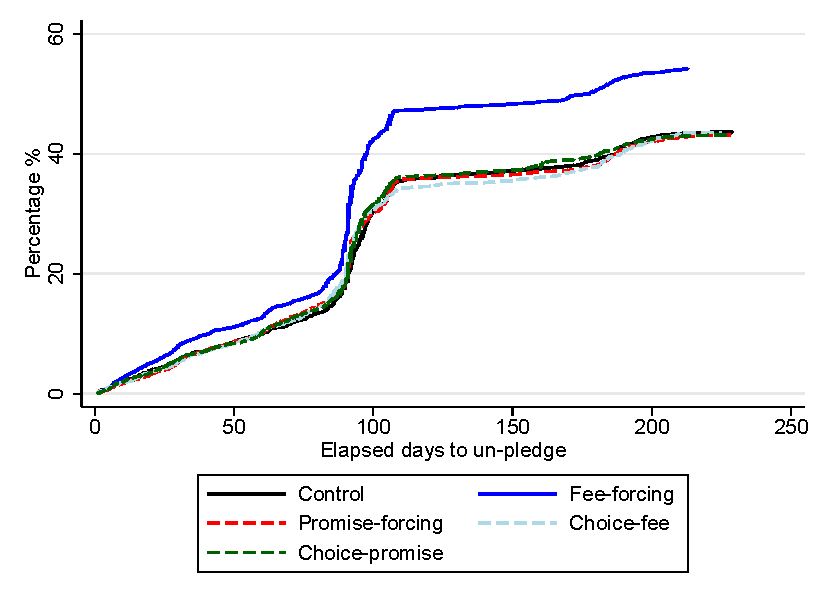
\includegraphics[width=0.75\textwidth]{Figuras/survival_graph_unpledge.pdf}
    \end{center}
\end{figure}   
\end{frame}


\begin{frame}{Censoring}
    \begin{table}[H]
\caption{Bounding censoring}
\label{bounding_censoring}
\begin{center}
\resizebox{0.9\textwidth}{!}{
\scriptsize{% Table generated by Excel2LaTeX from sheet 'censoring_imp_pres'
\begin{tabular}{lccccc}
\toprule
      & Control  = 0  & Control  = 0  & Control  = 1 & Control  = 1  & Prediction  \\
      & Forced arm = 0 & Forced arm = 1 & Forced arm = 0 & Forced arm = 1 & model \\
\midrule
      & \multicolumn{5}{c}{Financial Cost} \\
\midrule
      & (1)   & (2)   & (3)   & (4)   & (5) \\
\midrule
\midrule
Forced commitment  & -408.7*** & -226.5** & -804.2*** & -622.0*** & -525.3*** \\
      & (107.1) & (110.8) & (113.3) & (117.3) & (122.0) \\
      &       &       &       &       &  \\
\midrule
Observations & 3724  & 3724  & 3724  & 3724  & 3724 \\
R-sq  & 0.012 & 0.009 & 0.022 & 0.015 & 0.012 \\
Control Mean & 1898.5 & 1898.5 & 2272.4 & 2272.4 & 2073.6 \\
\midrule
\midrule
      &       &       &       &       &  \\
\midrule
      & \multicolumn{5}{c}{Default} \\
\midrule
\midrule
      & (6)   & (7)   & (8)   & (9)   & (10) \\
\midrule
\midrule
Forced commitment  & -0.063*** & 0.0089 & -0.21*** & -0.13*** & -0.12*** \\
      & (0.023) & (0.024) & (0.023) & (0.024) & (0.025) \\
      &       &       &       &       &  \\
\midrule
Observations & 3724  & 3724  & 3724  & 3724  & 6304 \\
R-sq  & 0.019 & 0.014 & 0.053 & 0.028 & 0.016 \\
Control Mean & 0.44  & 0.44  & 0.57  & 0.57  & 0.51 \\
\bottomrule
\bottomrule
\end{tabular}%
}
}
\end{center}
 \scriptsize 
%\textit{Do file: } \texttt{censoring_imp.do, censoring_imp_pr.do}
\end{table}
\end{frame}


\begin{frame}{Interpolation on bounding censoring}
    
\begin{figure}[H]
        \caption{Significance area for Default}
    \label{interpolation_censoring_imp}
    \begin{center}
        \includegraphics[width=0.75\textwidth]{Figuras/frontera_sig_def_imp.pdf}
    \end{center}
\end{figure}
\end{frame}


\begin{frame}{Bounding Individual Treatment Effects}
\label{fan_park_bounds}    

\begin{figure}[H]
    \caption{Fan \& Park bounds for benefit in effective FC }
    
    \begin{center}
        \includegraphics[width=0.75\textwidth]{Figuras/fan_park_bounds_fc_admin.pdf}
    \end{center}
   
\end{figure}
 \hyperlink{choice_hte}{\beamerbutton{Back}}
\end{frame}



\begin{frame}{The `Randomized Choice' Design}
\label{rc_design}
\begin{itemize}
    \vfill \item  Large literature estimating ToT and TuT to better understand who selects  into  treatment  and  why : \begin{itemize}
        \item “LATE-and-reweight" : Aronow \& Carnegie (2013); Angrist \& Fernandez—Val (2013)  - no selection on gains.  
        \item Cornelissen et. al. (2018); Walters (2018)  - Modeling assumptions to extrapolate from the reduced-form quantities
        %TUT and ATE implied by LATE-and-reweight differ sharply from his model-based estimates
        \item Heckman \& Vytlacil MTE - no parametric  restrictions,  but  an  instrumental  variable $Z$ with sufficiently rich support.
        \item Brinch et. al. (2017) - discrete $Z$ but under some additivity restrictions on the MTE curve
        \item Mogstad, Santos \& Torgovitsky (2018) - No parametric form assumption on MTE curve but only partial identification.
    \end{itemize}
    
    \vfill \item Our “randomized choice design,” point identifies a number of interesting and economically-relevant causal quantities  without  the  need  for  additional  structural  restrictions.  \hyperlink{identification_randomized_choice}{\beamerbutton{Identification}} %Only assuming mean exclusion
    \hyperlink{choice_hte}{\beamerbutton{Back}}
\end{itemize}
\end{frame}


\begin{frame}{Causal Parameters}
\begin{table}[H]
\caption{Causal TE}
\label{tot_tut}
\begin{center}
\scriptsize{% Table generated by Excel2LaTeX from sheet 'tot_tut_pres1'
\begin{tabular}{lcc}
\toprule
      & FC benefit & \% (1-Default) \\
\midrule
      & (1)   & (2) \\
\midrule
\midrule
ToT   & 668.3 & 38.7* \\
      & (1085.4) & (21.5) \\
TuT   & 356.1*** & 3.98* \\
      & (107.8) & (2.40) \\
\midrule
ToT-TuT & 312.2 & 34.7 \\
      & (1132.4) & (22.5) \\
ASB   & -77.9 & -40.6* \\
      & (1127.5) & (22.2) \\
ASL   & 234.3 & -5.90 \\
      & (154.4) & (4.29) \\
      &       &  \\
\midrule
Observations & 6304  & 6304 \\
\bottomrule
\bottomrule
\end{tabular}%
}
\end{center}
\end{table}

\begin{itemize}
    \item Commitment is beneficial to people who would not choose it. 
    \item The “right people” choose to commit:  those who are most likely to benefit from it and those whose outcomes are most adverse under the status quo.
\end{itemize}
 
\end{frame}

 
 
\begin{frame}{Identification of treatment parameters}
\label{identification_randomized_choice}
\begin{equation*}
    Y_i = \mathbbm{1}(Z_i =0) Y_{i0} + \mathbbm{1}(Z_i = 1)  Y_{i1}  + \mathbbm{1}(Z_i = 2) \left[(1 - C_i) Y_{i0} + C_i Y_{i1} \right].
\label{eq:potentialOutcomes}
\end{equation*}

    Viewing $Z_i$ as an instrumental variable, the randomized choice design can be interpreted as a \emph{pair} of RCTs, each subject to one-sided non-compliance. \\
    \begin{itemize}
        \item The first of these compares $Z_i=0$ to $Z_i = 2$.  This setting is identical to a ``randomized encouragement'' design in which treatment is only available to those who are encouraged: $Z_i = 2$. Under this interpretation, those with $C_i = 1$ are ``the compliers'' and it follows that 
\begin{equation*}
\frac{\mathbbm{E}(Y_i|Z_i=2) - \mathbbm{E}(Y_i|Z_i =0)}{\mathbbm{E}(D_i|Z_i=2)-\mathbbm{E}(D_i|Z_i=0)}  = \mathbbm{E}(Y_{i1} - Y_{i0}|C_i = 1)
\label{eq:ToT}
\end{equation*}

\item The second considers $Z_i = 1$ to be the ``encouragement'' and compare the outcomes for these individuals to those with $Z_i = 2$.
\begin{equation*}
\frac{\mathbbm{E}(Y_i|Z_i=1) - \mathbbm{E}(Y_i|Z_i =2)}{\mathbbm{E}(D_i|Z_i=1)-\mathbbm{E}(D_i|Z_i=2)}  = \mathbbm{E}(Y_{i1} - Y_{i0} | C_i = 0)
\label{eq:TuT}
\end{equation*}
    \end{itemize}

\hyperlink{rc_design}{\beamerbutton{Back}}


\end{frame}



\begin{frame}{If commitment works, why don't people choose it?}
\label{explanations_detailed}
    \begin{itemize}
         \onslide<1>{\item Discounting}
         \onslide<2>{\item Hyperbolicity}
          \onslide<3>{\item Overconfidence}
    \end{itemize}

\only<1>{  
\begin{figure}[H]
        \caption{Financial cost for different discount rates}
    \label{fc_discount_rates}
    \begin{center}
        \centering
        \includegraphics[width=0.45\textwidth]{Figuras/discount_effect.pdf}
    \end{center}
\end{figure}   
    \begin{itemize}
    \item   Commitment contract imposes up-front costs for later benefits (collateral recovery).  
    \item Can impatience explain why not take up a contract that decreases overall cost?
    \item  Requires a rate of ~2,000\% to make NPV cost effect insignificant. 
    \end{itemize}
}

\only<2>{  
  
    \begin{itemize}
   \vfill \item   Standard behavioral angle:  compliers are sophisticated time-inconsistent, non-compliers are a mix of naifs and the time consistent (who don't need commitment).  
   \vfill \item We have survey measure of time inconsistency taken at baseline.
   \vfill \item  Effect of Forcing should be entirely among the time-inconsistent.  Is this true? 
    \end{itemize}
}

\only<3>{  
  
    \begin{itemize}
   \vfill \item   Asked question prior to assignment, borrowing about subjective probability of recovering.  
   \vfill \item Mean of prior prediction is XX\%, true recovery in control is YY\%.
   \vfill \item  Use prediction of default in control, subjective priors to measure overconfidence.  Does this explain large TUT? 
    \end{itemize}
}

\hyperlink{explanations}{\beamerbutton{Back}}


\end{frame}




\begin{frame}{Paternalism and learning}
    

    \begin{itemize}
    \item   Are those with a greater experience of pawning less over-confident?  
    \begin{itemize}
        \item Observational analysis of overconfidence by number of prior pawns.
    \end{itemize}  
    \item   Do people learn from Forced exposure to the program that they benefit from it?  
    \begin{itemize}
        \item Subsequent to the experimental loan, those exposed to different treatments returned to branches where they were offered Choice.  What did they do?
    \end{itemize}  

    \end{itemize}     

    
\end{frame}


\end{document}






